\documentclass{../tuda-beamer}

% Packages
\usepackage{algorithm}
\usepackage{algpseudocode}

% Title information
\authors{Simon Hock}
\authors{Nhan Huynh}
\authors{Daniel Mangold}
\date{15. Dezember 2021}

% Tikz
\usetikzlibrary{mindmap}

% Commands
\NewDocumentCommand{\highlight}{m}{
    \colorbox{TUDa-8b!20}{#1}
}

% Document
\begin{document}

    \maketitle

    \begin{frame}[c]{Hinweis}
        \begin{center}
            12.01.2022 Präsenzsprechstunde B im Raum in Raum S103/\textbf{123}!
        \end{center}
    \end{frame}

    \begin{frame}{Überblick}
        \tableofcontents
    \end{frame}


    \section{Rekursion [25min]}
    \begin{frame}[c]{Rekursion}
        \begin{center}
            \enquote{Eine Rekursion ist eine Funktion, die sich selbst aufruft. Dabei wird versucht
            das Problem auf eine einfachere Variante des \textbf{gleichen} Problems rekursiv zu
            reduzieren, welches dann gelöst wird.}
        \end{center}
    \end{frame}

    \subsection{Vorgehensweise bei rekursiven Aufgaben}
    \begin{frame}{Vorgehensweise bei rekursiven Aufgaben}
        \begin{enumerate}
            \item Identifiziere, wie das Problem auf eine einfachere Variante des Problems
            zerlegt werden kann und direkt gelöst werden kann

            \begin{itemize}
                \item Teillösungen der Gesamtlösung
            \end{itemize}
            \item Das kleinste Problem ist ein Rekursionsanker
            \item Überlege, wie die kleinen Problemen kombiniert werden können, um die
            ursprüngliche Problemstellung zu lösen
            \item Kombiniere die Teillösungen zu einer Gesamtlösung
        \end{enumerate}
    \end{frame}

    \subsection{Rekursive Auswertung von Arithmetischen Ausdrücken in Präfix-Notation}
    \begin{frame}{Rekursive Auswertung von Arithmetischen Ausdrücken in Präfix-Notation}
        \begin{itemize}
            \item \href{https://moodle.informatik.tu-darmstadt.de/pluginfile.php/202303/mod_resource/content/3/uebung06.pdf}{Blatt 06 H4}
            \item Prfäix-Notation Beispiele:
            \begin{itemize}
                \item \(+ 2 \ 3 = 5\)
                \item \(* - 1 2 3 = * (-1 2) 3 = - 3\)
                \item \(+ 4 - 5 1 = + 4 (- 5 1) = 8\)
            \end{itemize}
        \end{itemize}

        \begin{table}[h]
            \rowcolors{2}{white}{gray!25}
            \centering
            \begin{tabular}{lc}
                \toprule
                \textbf{Notation} & \textbf{Addition zweier Zahlen}
                \\
                \midrule
                Präfix & \(+ \ x \ y\)
                \\
                Infix & \(\ x + y\)
                \\
                Postfix & \(x \ y \ +\)
                \\
                \bottomrule
            \end{tabular}
            \caption{Überblick von Notationen}
        \end{table}
    \end{frame}

    \begin{frame}[c]{H4.1: Vorbereitung: Klasse \inlinejava{ReturnData}}
        Schreiben Sie zunächst eine eine \inlinejava{public}-Klasse
        \highlight{\inlinejava{ReturnData}}, welche zwei
        \inlinejava{public}-\highlight{Objektattribute} vom Typ \highlight{\inlinejava{int}} hat:
        \highlight{\inlinejava{result}} und \highlight{\inlinejava{nextIndex}}. Diese Klasse muss
        einen \highlight{parameterlosen} \inlinejava{public}-\highlight{Konstruktor} besitzen.
        Sie dürfen aber gerne auch andere Konstruktoren implementieren, solange weiterhin ein
        parameterloser \inlinejava{public}-Konstruktor zur Verfügung steht.
    \end{frame}

    \begin{frame}
        \lstinputlisting[style=Java]{codes/ReturnData.java}
    \end{frame}

    \begin{frame}[c]{H4.2: Methoden \inlinejava{evaluate} und \inlinejava{evaluateRecursively}}
        Erweitern Sie Klasse \inlinejava{StrangeThings} aus 2 um eine
        \inlinejava{public}-\highlight{Klassenmethode \inlinejava{evaluate}}, die den Wert eines
        \highlight{arithmetischen Ausdrucks} in \highlight{Präfix-Notation} (das heißt: zuerst
        Operator, dann Operanden) berechnet. Es geht also um eine Notation wie in Racket -- aber
        im Gegensatz zu Racket haben wir \highlight{keine Klammern}. Außerdem beschränken wir uns
        bei den Operanden auf \highlight{einstellige Zahlen} (also \(0 \dots 9\))) und bei dem
        Operator um die \highlight{Subtraktion}.

        \vskip 2em

        \begin{note}[title=Information:, color=tuda-orange]
            \enquote{Ein arithmetischer Ausdruck besteht aus einer Folge von arithmetischen
            Operanden, die durch (arithmetische) Operatoren und Klammern voneinander getrennt
                (oder miteinander verknüpft) sind.}
        \end{note}
    \end{frame}

    \begin{frame}{Beispiel für arithmetische Ausdrücke}
        \begin{align}
            1
            \\
            - \ 1 \ 2
            \\
            - \ - \ 1 \ 2 \ 3
            \\
            - \ - \ 1 \ 2 \ - \ 3 \ 4
        \end{align}
    \end{frame}

    \begin{frame}
        \setcounter{equation}{0}
        \begin{align}
            1
            \\
            \underbrace{- \ 1 \ 2}_{1 - 2 = -1}
            \\
            \underbrace{- \ \underbrace{- \ 1 \ 2}_{1 - 2 = -1} \ 3}_{-1 - 3 = -4}
            \\
            \underbrace{- \ \underbrace{- \ 1 \ 2}_{1 - 2 = -1} \underbrace{- \ 3 \ 4}_{3 - 4 =
            -1}}_{-1 - (-1) = 0}
        \end{align}
    \end{frame}

    \begin{frame}[c]
        Konkret hat Methode \inlinejava{evaluate} einen Parameter vom formalen Typ
        \enquote{\highlight{Array} vom primitiven Typ \highlight{\inlinejava{char}}} und Rückgabetyp
        \highlight{\inlinejava{int}}. Die Methode \inlinejava{evaluate} darf ohne Überprüfung
        davon ausgehen, dass das Array \highlight{mindestens die Länge 1} hat und jede Komponente
        des Arrays entweder \highlight{eine Ziffer \inlinejava{'0'}, \dots, \inlinejava{'9'} oder
        das Zeichen \inlinejava{'-'}} enthält und der mit der \inlinejava{char}-Kette
        repräsentierte Präfix-Ausdruck ein korrekt gebildeteter Präfix-Ausdruck ist, in dem
        \highlight{jede Subtraktion genau zwei Operanden} hat.

        \pause

        \vskip 1em

        \begin{note}[title=Information:]
            Beim Parameterwert wird zwischen dem aktualen Wert (der Parameterwert, der eingesetzt
            wird) und dem formalen Wert (der in der Definition des Parameters in der Methode
            steht) unterschieden.
        \end{note}
    \end{frame}

    \begin{frame}[c]
        Neben der Methode \inlinejava{evaluate} soll in Klasse \inlinejava{StrangeThings} eine
        \inlinejava{private}-\highlight{Klassenmethode}
        \highlight{\inlinejava{evaluateRecursively}} mit einem ersten Parameter namens
        \highlight{\inlinejava{array}} vom Typ \enquote{\highlight{Array} vom primitiven Typ
        \highlight{\inlinejava{char}}}, einem zweiten Parameter namens
        \highlight{\inlinejava{startIndex}} vom Typ \highlight{\inlinejava{int}} und Rückgabetyp
        \highlight{\inlinejava{ReturnData}} existierten.

        \vskip 1em

        Die Methode \inlinejava{evaluateRecursively} soll aus dem Array \inlinejava{array} den
        \highlight{numerischen (Teil-)Ausdruck} \highlight{ab Index \inlinejava{startIndex}
        auswerten} und ein \highlight{\inlinejava{ReturnData}}-Objekt zurückliefern, dessen
        Objekt- \\attribut \highlight{\inlinejava{result}} den Zahlenwert des ausgewerteten
        numerischen (Teil-) Ausdrucks ab Index \inlinejava{startIndex} und Objektattribut
        \highlight{\inlinejava{nextIndex}} den ersten Index des nächsten numerischen
        Teilausdrucks enthält.
    \end{frame}

    \begin{frame}[c]
        Die Methode \inlinejava{evaluate} ruft die Methode
        \highlight{\inlinejava{evaluateRecursively}} auf, wobei \inlinejava{evaluateRecursively}
        als ersten aktualen Parameter den \highlight{ersten aktualen Parameter von}
        \highlight{\inlinejava{evaluate}} erhält (beides jeweils \enquote{\highlight{Array} von
        \highlight{\inlinejava{char}}}). Als zweiten aktualen Parameter erhält
        \inlinejava{evaluateRecursively} den Wert \highlight{\inlinejava{0}}. Nach dem Aufruf von
        \inlinejava{evaluateRecursively} liefert die Methode \inlinejava{evaluate} den Wert des
        Objektattributs \highlight{\inlinejava{result}} des von \inlinejava{evaluateRecursively}
        gelieferten Objekts vom Typ \highlight{\inlinejava{ReturnData}}.
    \end{frame}

    \begin{frame}[c]
        Das Verhalten der Methode \inlinejava{evaluateRecursively} ist vom Zeichen am Index
        \highlight{\inlinejava{startIndex}} in Array \inlinejava{array} abhängig:

        \vskip 1em

        Im Fall, dass der \inlinejava{char}-Wert \highlight{\inlinejava{array[startIndex]}} eine
        \highlight{Ziffer} darstellt, wurde ein \highlight{atomarer arithmetischer Ausdruck}
        gefunden und die Methode liefert ein \highlight{\inlinejava{ReturnData}}-Objekt zurück,
        dessen Objektattribut \highlight{\inlinejava{result}} den durch das \highlight{Zeichen
        dargestellten Wert} (für \inlinejava{'4'} zum Beispiel \inlinejava{4})
        und \highlight{\inlinejava{nextIndex}} den Wert \highlight{\inlinejava{startIndex+1}}
        enthält.

        \vskip 1em

        Im anderen Fall, also wenn der \inlinejava{char}-Wert gleich \highlight{\inlinejava{'-'}}
        ist, müssen die  \highlight{nächsten beiden arithmetischen Teil-Ausdrücke}
        \inlinejava{e1} und \inlinejava{e2} \highlight{ausgewertet} und
        ein geeignetes \highlight{\inlinejava{ReturnData}}-Objekt zurückgegeben werden.

        \vskip 1em

        Implementieren Sie die Methoden \inlinejava{evaluate} und
        \inlinejava{evaluateRecursively} wie beschrieben.
    \end{frame}

    \begin{frame}[c]
        \begin{itemize}
            \item \inlinejava{array}: Enthält den arithmetischen Ausdruck, bspw.
            \inlinejava{['-', '1', '2']}
            \item \inlinejava{startIndex}: Aktualler Index beim Durchlauf durch das Array
            \inlinejava{array}
            \item \inlinejava{ReturnData}
            \begin{itemize}
                \item \inlinejava{result}: Enthält das Ergebnis des bisher berechneten Teilausdrucks
                \item \inlinejava{nextIndex}: Gibt den ersten Index des nächsten Teilausdrucks an
            \end{itemize}
        \end{itemize}

        \vskip 1em

        \lstinputlisting[style=Java]{codes/evaluate_02.java}
    \end{frame}

    \begin{frame}[c]
        \begin{itemize}
            \item Hauptrekursion wird in der Hilfsmethode \inlinejava{evaluateRecursively}
            durchgeführt
            \item \inlinejava{ReturnData} enthält das Ergebnis der Auswertung
        \end{itemize}

        \lstinputlisting[style=Java]{codes/evaluate_03.java}
    \end{frame}

    \begin{frame}
        \begin{enumerate}
            \item Identifiziere, wie das Problem auf eine einfachere Variante des Problems
            zerlegt werden kann und direkt gelöst werden kann
        \end{enumerate}

        \begin{figure}[h]
            \centering
            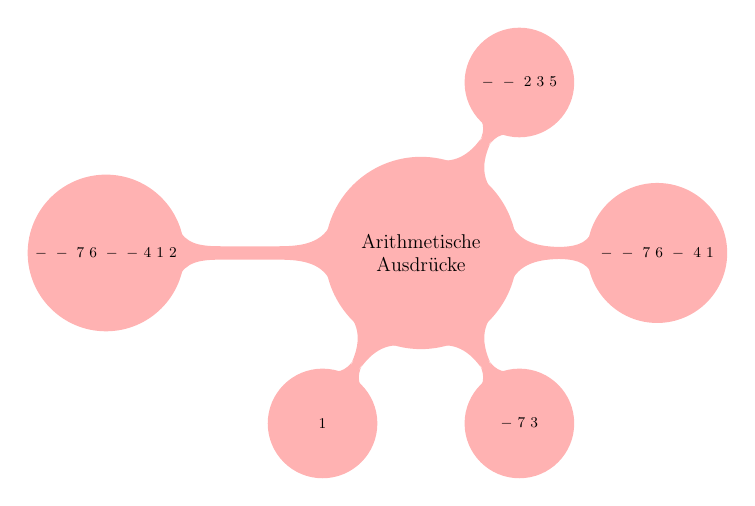
\begin{tikzpicture}[
                mindmap,
                concept color=red!30,
                every node/.style={concept, scale=0.6},
                grow cyclic,
                level 1/.append style={
                level distance=2.5cm,
                sibling angle=60,
                },
            ]
                \node {Arithmetische Ausdrücke}
                child {
                    node {
                        \(1\)
                    }
                }
                child {
                    node {
                        \(- \ 7 \ 3\)
                    }
                }
                child[level distance=3cm]  {
                    node[text width=8em] {
                        \(- \ - \ 7 \ 6 \ - \ 4 \ 1\)
                    }
                }
                child {
                    node {
                        \(- \ - \ 2 \ 3 \ 5\)
                    }
                }
                child[grow=left, level distance=4cm] {
                    node[text width=9em] {
                        \(- \ - \ 7 \ 6 \ - \ -  \ 4 \ 1 \ 2\)
                    }
                };
            \end{tikzpicture}
        \end{figure}
    \end{frame}

    \begin{frame}
        \begin{enumerate}
            \item Identifiziere, wie das Problem auf eine einfachere Variante des Problems
            zerlegt werden kann und direkt gelöst werden kann
        \end{enumerate}

        \begin{figure}[h]
            \centering
            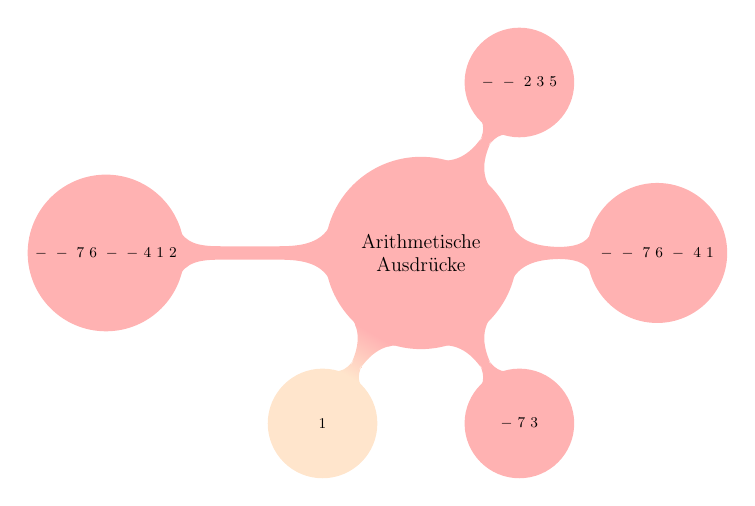
\begin{tikzpicture}[
                mindmap,
                concept color=red!30,
                every node/.style={concept, scale=0.6},
                grow cyclic,
                level 1/.append style={
                level distance=2.5cm,
                sibling angle=60,
                },
            ]
                \node {Arithmetische Ausdrücke}
                child[concept color=orange!20] {
                    node {
                        \(1\)
                    }
                }
                child {
                    node {
                        \(- \ 7 \ 3\)
                    }
                }
                child[level distance=3cm]  {
                    node[text width=8em] {
                        \(- \ - \ 7 \ 6 \ - \ 4 \ 1\)
                    }
                }
                child {
                    node {
                        \(- \ - \ 2 \ 3 \ 5\)
                    }
                }
                child[grow=left, level distance=4cm] {
                    node[text width=9em] {
                        \(- \ - \ 7 \ 6 \ - \ -  \ 4 \ 1 \ 2\)
                    }
                };
            \end{tikzpicture}
        \end{figure}
    \end{frame}

    \begin{frame}
        \begin{enumerate}
            \setcounter{enumi}{1}
            \item Das kleinste Problem ist ein Rekursionsanker
        \end{enumerate}

        \begin{algorithm}[H]
            \caption{evaluateRecursively(array, startIndex)}
            \begin{algorithmic}[1]
                \If{array[startIndex] is a digit}
                    \State \Return array[startIndex], startIndex + 1
                \EndIf
            \end{algorithmic}
        \end{algorithm}
    \end{frame}

    \begin{frame}[c]
        \lstinputlisting[style=Java]{codes/evaluate_04.java}
    \end{frame}

    \begin{frame}
        \begin{enumerate}
            \setcounter{enumi}{2}
            \item Überlege, wie die kleinen Problemen kombiniert werden können, um die
            ursprüngliche Problemstellung zu lösen
        \end{enumerate}

        \begin{equation*}
            \underbrace{\text{1. kleines Problem und 2. kleines Problem}}_{\text{Kombinieren}}
        \end{equation*}

        \begin{itemize}
            \item Wann werden die beiden Probleme zusammengefügt? \pause \(\Rightarrow\) Wenn ein
            Operator gelesen wird
        \end{itemize}

        \begin{algorithm}[H]
            \caption{evaluateRecursively(array, startIndex)}
            \begin{algorithmic}[1]
                \If{array[startIndex] is a digit}
                    \State \Return array[startIndex], startIndex + 1
                \Else
                    \State leftOperand \(\leftarrow\) evaluateRecursively(array, \dots)
                    \State rightOperand \(\leftarrow\) evaluateRecursively(array, \dots)
                    \State \Return leftOperand.result + rightOperand.result, \dots
                \EndIf
            \end{algorithmic}
        \end{algorithm}
    \end{frame}

    \begin{frame}
        \begin{itemize}
            \item Von welchen Indizes starten die Operanden bzw. was ist der nächste Index nach
            der Kombination?
        \end{itemize}

        \begin{algorithm}[H]
            \caption{evaluateRecursively(array, startIndex)}
            \begin{algorithmic}[1]
                \If{array[startIndex] is a digit}
                    \State \Return array[startIndex], startIndex + 1
                \Else
                    \State leftOperand \(\leftarrow\) evaluateRecursively(array, \dots)
                    \State rightOperand \(\leftarrow\) evaluateRecursively(array, \dots)
                    \State \Return leftOperand.result + rightOperand.result, \dots
                \EndIf
            \end{algorithmic}
        \end{algorithm}
    \end{frame}

    \begin{frame}
        \begin{figure}[h]
            \begin{tikzpicture}
                \begin{scope}[
                    every node/.style={
                    align=center,
                    draw,
                    minimum height=.5cm,
                    minimum width=.5cm,
                    node distance=0pt,
                    rectangle,
                    },
                ]
                    \node (0) {--};
                    \node[right=of {0}] (1) {--};
                    \node[right=of {1}] (2) {1};
                    \node[right=of {2}] (3) {2};
                    \node[right=of {3}] (4) {--};
                    \node[right=of {4}] (5) {3};
                    \node[right=of {5}] (6) {4};
                \end{scope}

                \node[below left=3.5cm and 1cm of {0}] (op1) {Operator};
                \node[below=of {1}] (op2) {Operator};
                \node[below=of {4}] (op3) {Operator};
                \node[below=of {op1}] (exp1) {Ausdruck};
                \node[below=of {op2}] (exp2) {Ausdruck};
                \node[below=of {op3}] (exp3) {Ausdruck};

                \draw[-latex] (0.south) -- (op1.north);
                \draw[-latex] (1.south) -- (op2.north);
                \draw[-latex] (4.south) -- (op3.north);

                \draw[-latex] (op2.north) -- (2.south);
                \draw[-latex] (op2.north) -- (3.south);

                \draw[-latex] (op3.north) -- (5.south);
                \draw[-latex] (op3.north) -- (6.south);

                \draw[-latex] (op1.south) -- (exp1);
                \draw[-latex] (op2.south) -- (exp2);
                \draw[-latex] (op3.south) -- (exp3);

                \draw[-latex] (op1.east) -- (exp2.south);
                \draw[-latex] (op1.east) -- (exp3.south);
            \end{tikzpicture}
            \caption{Visualisierung der Auswertung}
        \end{figure}
    \end{frame}

    \begin{frame}{Linker Operand}
        \begin{itemize}
            \item Wir müssen rekursiv den nächsten Index abprüfen
        \end{itemize}

        \begin{algorithm}[H]
            \caption{evaluateRecursively(array, startIndex)}
            \begin{algorithmic}[1]
                \If{array[startIndex] is a digit}
                    \State \Return array[startIndex], startIndex + 1
                \Else
                    \State leftOperand \(\leftarrow\) evaluateRecursively(array, startIndex + 1)
                    \State rightOperand \(\leftarrow\) evaluateRecursively(array, \dots)
                    \State \Return leftOperand.result + rightOperand.result, \dots
                \EndIf
            \end{algorithmic}
        \end{algorithm}
    \end{frame}

    \begin{frame}{Rechter Operand}
        \begin{itemize}
            \item Wir müssen rekursiv nach dem letzten besuchten Index von dem linken Operand
            abprüfen
        \end{itemize}

        \begin{algorithm}[H]
            \caption{evaluateRecursively(array, startIndex)}
            \begin{algorithmic}[1]
                \If{array[startIndex] is a digit}
                    \State \Return array[startIndex], startIndex + 1
                \Else
                    \State leftOperand \(\leftarrow\) evaluateRecursively(array, startIndex + 1)
                    \State rightOperand \(\leftarrow\) evaluateRecursively(array, leftOperand
                    .nextIndex)
                    \State \Return leftOperand.result + rightOperand.result, \dots
                \EndIf
            \end{algorithmic}
        \end{algorithm}
    \end{frame}

    \begin{frame}{Kombination}
        \begin{itemize}
            \item Der nächste Index nach der Kombination ist der Index nach der Auswertung von
            dem rechten Teilausdruck
        \end{itemize}

        \begin{algorithm}[H]
            \caption{evaluateRecursively(array, startIndex)}
            \begin{algorithmic}[1]
                \If{array[startIndex] is a digit}
                    \State \Return array[startIndex], startIndex + 1
                \Else
                    \State leftOperand \(\leftarrow\) evaluateRecursively(array, startIndex + 1)
                    \State rightOperand \(\leftarrow\) evaluateRecursively(array, leftOperand
                    .nextIndex)
                    \State \Return leftOperand.result + rightOperand.result, rightOperand.nextIndex
                \EndIf
            \end{algorithmic}
        \end{algorithm}
    \end{frame}

    \begin{frame}[c]
        \lstinputlisting[style=Java]{codes/evaluate_05.java}
    \end{frame}


    \section{Arbeitsphase [75min]}
    \begin{frame}[c]{Arbeitsphase}
        \begin{center}
            \textbf{\LARGE Selbstständiges Arbeiten}
        \end{center}
    \end{frame}
\end{document}
